\documentclass[conference]{IEEEtran}
\IEEEoverridecommandlockouts
% The preceding line is only needed to identify funding in the first footnote. If that is unneeded, please comment it out.
\usepackage{cite}
\usepackage{amsmath,amssymb,amsfonts}
\usepackage{algorithmic}
\usepackage{graphicx}
\usepackage{textcomp}
\usepackage{xcolor}
\usepackage{caption}
\usepackage{subcaption}
\usepackage{multirow}
\def\BibTeX{{\rm B\kern-.05em{\sc i\kern-.025em b}\kern-.08em
    T\kern-.1667em\lower.7ex\hbox{E}\kern-.125emX}}
\begin{document}

\title{Image Processing and Computer Vision\\
}
\author{\IEEEauthorblockN{1\textsuperscript{st} George Lancaster}
\IEEEauthorblockA{\textit{dept. of Computer Science} \\
\textit{University of Bristol}\\
Bristol, United Kingdom \\
qv18258@bristol.ac.uk}
\and
\IEEEauthorblockN{2\textsuperscript{nd} Ren Jiang}
\IEEEauthorblockA{\textit{dept. of Computer Science} \\
\textit{University of Bristol}\\
Bristol, United Kingdom \\
mu18336@bristol.ac.uk}
}


\maketitle

\begin{abstract}
This report outlines the tasks completed for Image Processing and Computer Vision assignment one. Our final classifier, which has been extended to do x, y and z has an F1 score of x.xx when tested against the 16 test images. 
\end{abstract}

\section{The Viola-Jones Object Detector}
Sixteen test images were annotated for ground truth. Each test image contains either faces, dartboards or a combination of both. In this first task, we use the Viola-Jones object detector to find faces within the test images. 
\begin{figure}[htb]
\centering
\begin{subfigure}{.5\linewidth}
  \centering
  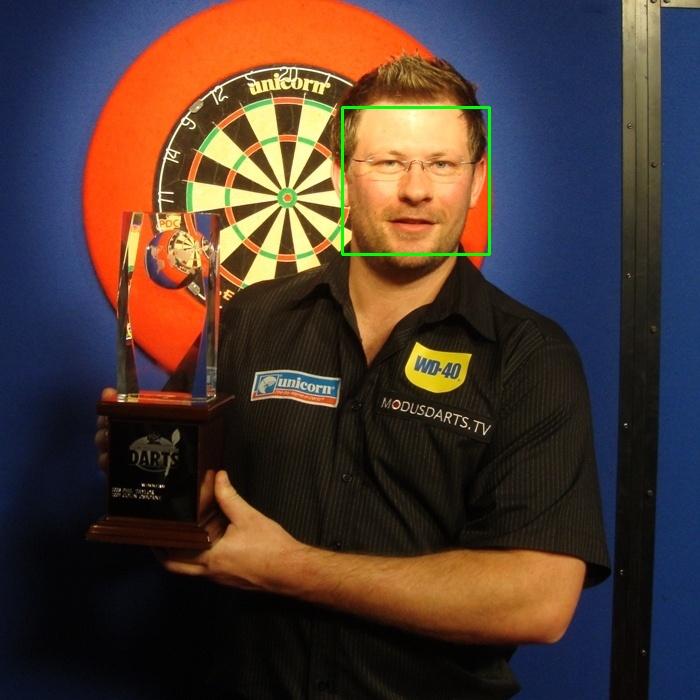
\includegraphics[width=.9\linewidth]{images/detected0.jpg}
  \caption{darts4.jpg}
  \label{fig:sub1}
\end{subfigure}%
\begin{subfigure}{.5\linewidth}
  \centering
  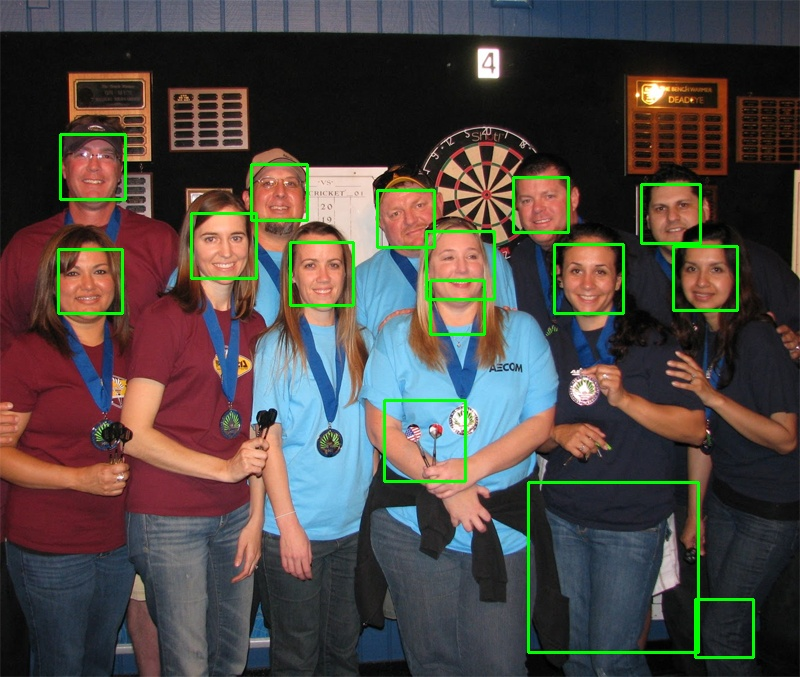
\includegraphics[width=.9\linewidth]{images/detected1.jpg}
  \caption{darts5.jpg}
  \label{fig:sub2}
\end{subfigure}
\begin{subfigure}{.5\linewidth}
  \centering
  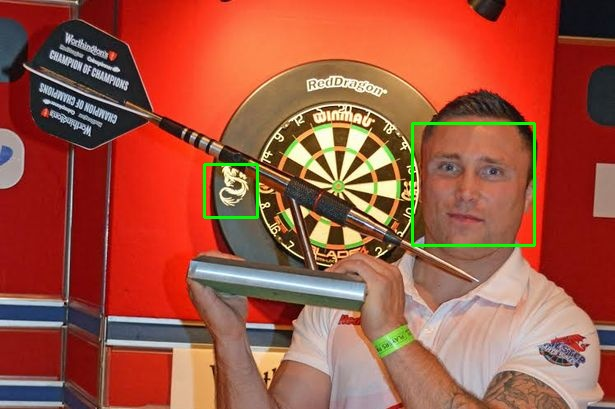
\includegraphics[width=.9\linewidth]{images/detected2.jpg}
  \caption{darts13.jpg}
  \label{fig:sub1}
\end{subfigure}%
\begin{subfigure}{.5\linewidth}
  \centering
  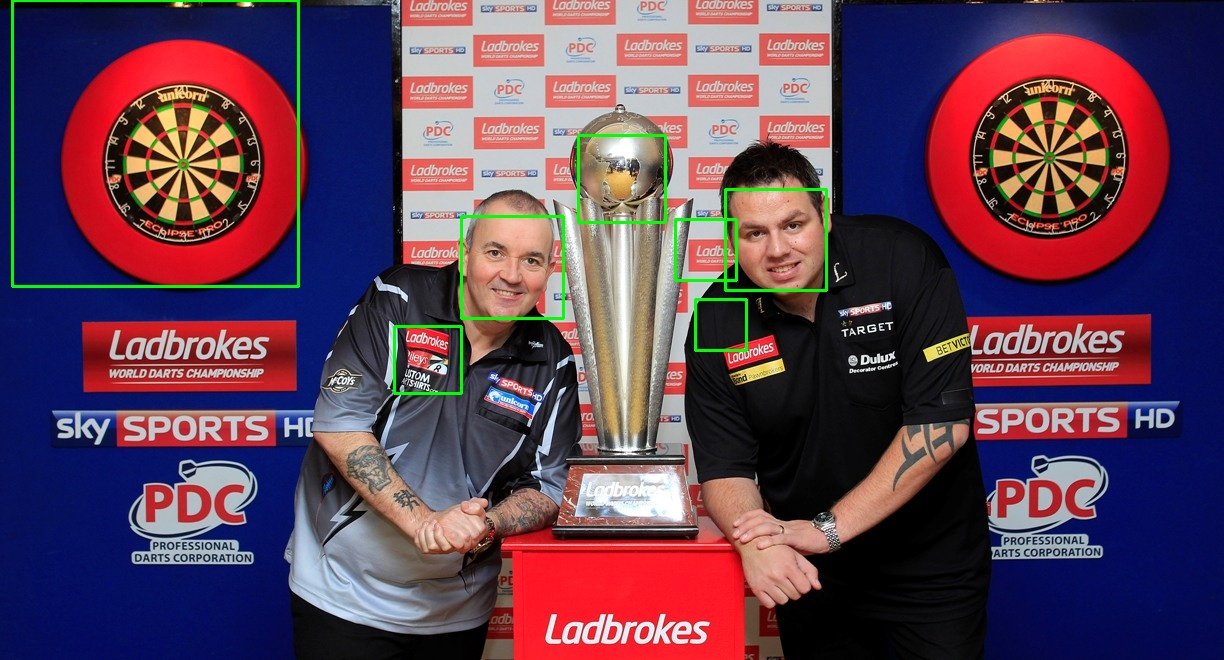
\includegraphics[width=.9\linewidth]{images/detected3.jpg}
  \caption{darts14.jpg}
  \label{fig:sub2}
\end{subfigure}
\begin{subfigure}{.5\linewidth}
\centering
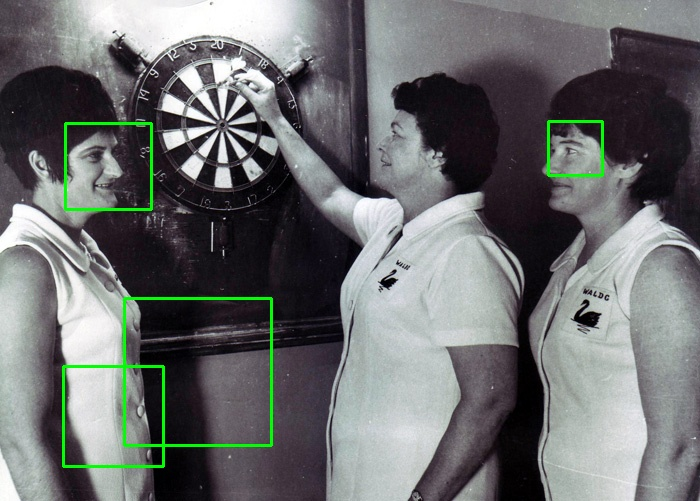
\includegraphics[width=0.9\linewidth]{images/detected4.jpg}
\caption{darts15.jpg}
\end{subfigure}


\caption{Five images from the test data set. Green rectangles have been drawn where the Viola-Jones classifier has detected a face. }
\label{fig:q13}
\end{figure}
\par 
The true positive rate for images \emph{darts5.jpg} and \emph{darts15.jpg} when tested using the Viola-Jones face detector are 1 and 0.667 respectively. 
\par
Although the true positive rate can be used to indicate a classifiers accuracy, it does not reflect its true performance. It is always possible to get a 100 per cent detection rate on any classification task as we can select all possible areas of an image, regardless if they contain the target feature or not. The key to a good classifier is to get a high true positive rate, whilst keeping the false positive rate minimal. The F1 score measures the relationship between the precision and the recall of the model and can therefore be considered to be a more reliable measure of classifier performance.
\par
The true positive rate can be difficult to assess as it requires the definition of a rule to determine what counts as a detection. For this task, a true detection is defined as an area that shares a 68 per cent overlap with a ground truth annotation. A value of 68 per cent was chosen as it is the largest area of overlap before the F1 score starts to decline. Table 1 shows how the F1 score changes when the percentage overlap area is changed.
\par 
\begin{table}[!htp]
\caption{All values of percentage overlap up to 68 per cent gave an identical F1 score when detecting faces from the test data set. This influenced the choice to set the overlap area to 68 per cent for this task. }
\begin{center}
\begin{tabular}{||c|c||}
\hline
Overlap Threshold (\%) 	& F1 score 	\\ \hline
0 					& 0.568		\\
60 					& 0.541		\\
65					& 0.541		\\
68					& 0.541		\\
69					& 0.519		\\
70 					& 0.514		\\
80					& 0.459		\\ \hline
\end{tabular}
\end{center}
\label{default}
\end{table}%
\par
Need more info here

\newpage
\section{The Dartboard Detector}
To detect dartboards, the Viola-Jones classifier was trained on a data set generated from a single bitmap image of a dartboard, as well as a set of negative images. 
\begin{figure}[htbp]
\begin{center}
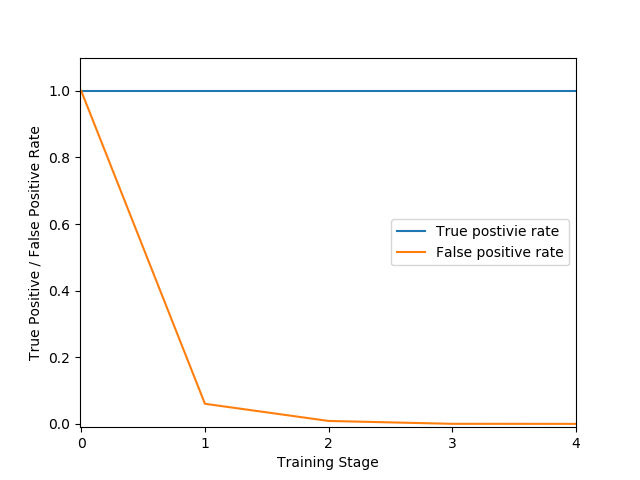
\includegraphics[width=\linewidth]{images/TPRvsFPR}
\caption{True positive rate plotted against false positive rate when training the cascade classifier on 500 images of dartboards and 500 negative images. Each stage of training has been plotted as its own point.}
\label{default}
\end{center}
\end{figure}
\par

On the first stage of training, all samples are classified as true. This is reflected by a value of 1 for both the true positive rate and false positive rate. As the classifier progresses through further training stages, the false positive rate decreases, whilst the true positive rate remains the same. This indicates that the classifier is improving after each training stage. 
\par
\begin{table}[!htb]
\caption{F1 scores for all images, when detecting for dartboards using a cascade classier trained on dartboards.}
\begin{center}
\begin{tabular}{||c|c|c||}
\hline
\multirow{2}{*}{Image Name} & \multicolumn{2}{c||}{F1 Score}                \\ 
                                 & 500 Training Images (a)	& 1000 Training images (b) \\ \hline
dart0.jpg			& 0.5	00	&	0.250	\\
dart1.jpg			& 0		&	0.500	\\
dart2.jpg			& 0.250	&	0.400	\\
dart3.jpg			& 0.538	&	0.333	\\
dart4.jpg			& 0.4	00	&	0.250	\\
dart5.jpg			& 0.154	&	0.200	\\
dart6.jpg			& 0.333	&	0.500	\\
dart7.jpg			& 0		&	0.250	\\
dart8.jpg			& 0.160	&	0.250	\\
dart9.jpg			& 0.222	&	0.200	\\
dart10.jpg			& 0.400	&	0.545	\\
dart11.jpg			& 0.222	&	0.222	\\
dart12.jpg			& 0.667	&	0.500	\\
dart13.jpg			& 0.200	&	0.333	\\
dart14.jpg			& 0.087	&	0.138	\\
dart15.jpg			& 0.667	&	0.500	\\ \hline
Average F1 score 	& 0.276	&	0.336	\\ \hline
\end{tabular}
\end{center}
\label{default}
\end{table}%
Two identical Viola-Jones classifiers were trained on sets of 500 (a), and 1000 (b) true images and negatives. The F1 score of classifier b was 0.06 higher than classifier a. 

\par
Observed differences in accuracy between training and testing can be attributed to the training data consisting of a small set of critical features. In contrast, the test images contain a large amount of irrelevant background noise, which needed to be discarded by the cascade. 

\par
\begin{figure}[htb]
\centering
\begin{subfigure}{.5\linewidth}
  \centering
  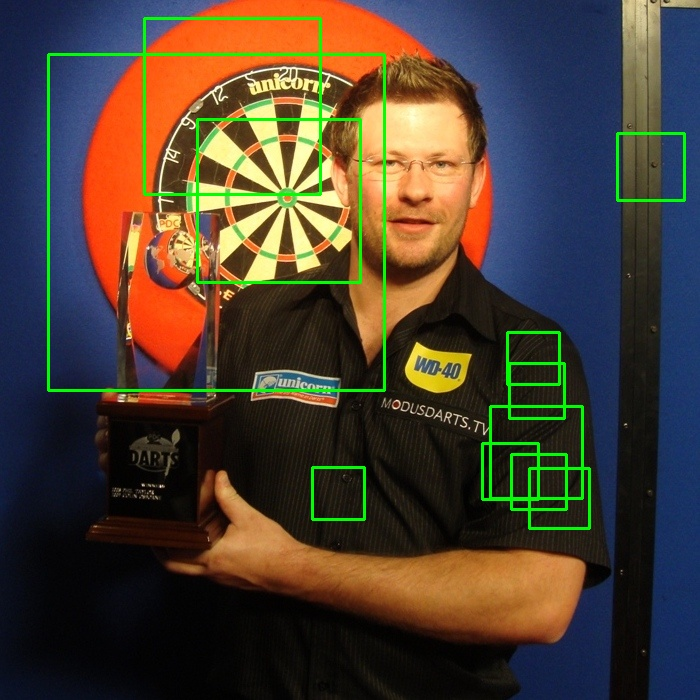
\includegraphics[width=.9\linewidth]{images/task2/detected4.jpg}
  \caption{darts4.jpg}
  \label{fig:sub1}
\end{subfigure}%
\begin{subfigure}{.5\linewidth}
  \centering
  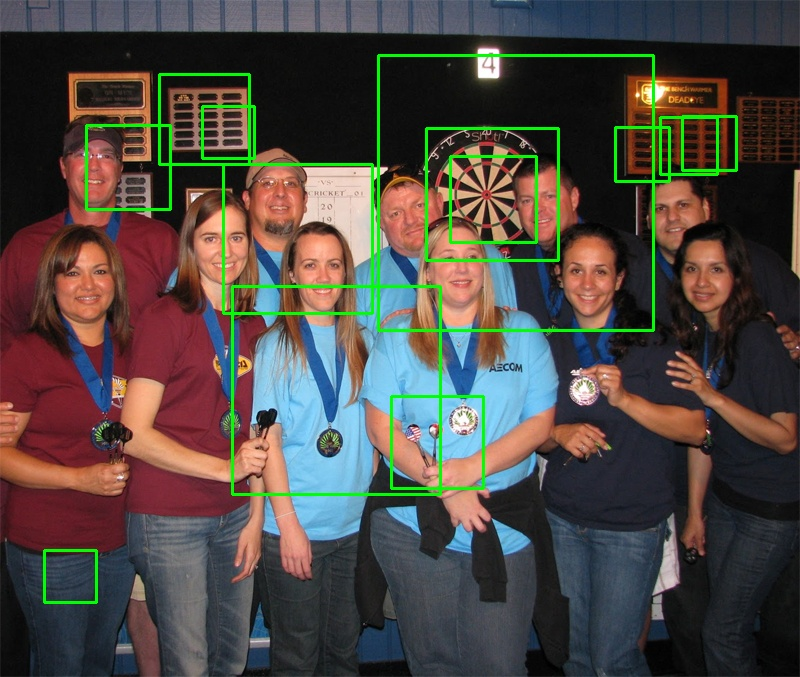
\includegraphics[width=.9\linewidth]{images/task2/detected5.jpg}
  \caption{darts5.jpg}
  \label{fig:sub2}
\end{subfigure}
\begin{subfigure}{.5\linewidth}
  \centering
  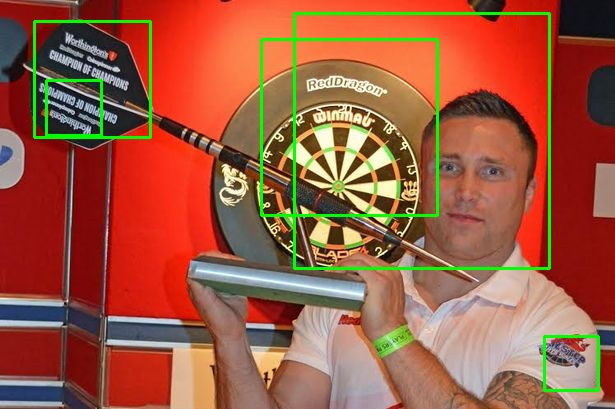
\includegraphics[width=.9\linewidth]{images/task2/detected13.jpg}
  \caption{darts13.jpg}
  \label{fig:sub1}
\end{subfigure}%
\begin{subfigure}{.5\linewidth}
  \centering
  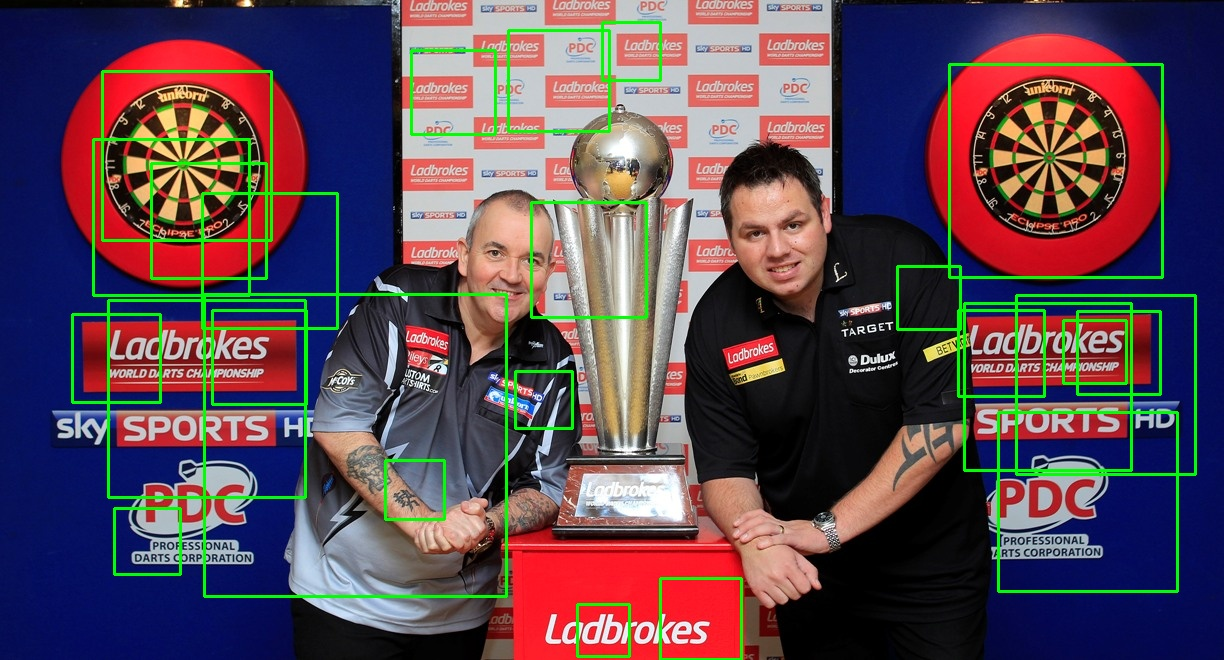
\includegraphics[width=.9\linewidth]{images/task2/detected14.jpg}
  \caption{darts14.jpg}
  \label{fig:sub2}
\end{subfigure}
\caption{Five images from the test data set. Green rectangles have been drawn where the Viola-Jones classifier has detected a dartboard.}
\end{figure}
\par

\newpage
\section{Integration with Shape Detectors}
Both linear and circular hough transforms have been used in conjunction with the Viola-Jones classifier to improve accuracy. 
\begin{table}[htp]
\caption{F1 scores, precision and recall for all images, when detecting for dartboards using the cascade classier combined with shape detection techniques. }
\begin{center}
\begin{tabular}{||c|c|c|c||}
\hline
Image Name			 	& F1 Score 	& Precision	& Recall            \\ \hline
dart0.jpg					& 1.000		&	1.000	& 1.000		\\
dart1.jpg					& 1.000		&	1.000	& 1.000		\\
dart2.jpg					& 1.000		&	1.000	& 1.000		\\
dart3.jpg					& 0.333		&	0.200	& 1.000		\\
dart4.jpg					& 1.000		&	1.000	& 1.000		\\
dart5.jpg					& 1.000		&	1.000	& 1.000		\\
dart6.jpg					& 1.000		&	1.000	& 1.000		\\
dart7.jpg					& 1.000		&	1.000	& 1.000		\\
dart8.jpg					& 1.000		&	1.000	& 1.000		\\
dart9.jpg					& 0.000		&	0.000	& 0.000		\\
dart10.jpg					& 1.000		&	1.000	& 1.000		\\
dart11.jpg					& 0.222		&	0.125	& 1.000		\\
dart12.jpg					& 0.667		&	0.500	& 1.000		\\
dart13.jpg					& 1.000		&	1.000	& 1.000		\\
dart14.jpg					& 0.500		&	0.333	& 1.000		\\
dart15.jpg					& 0.667		&	0.500	& 1.000		\\ \hline
Average 		 			& 0.774		&	0.729	& 0.938 		\\ \hline
\end{tabular}
\end{center}
\label{default}
\end{table}


\begin{figure}[htbp]
\begin{center}
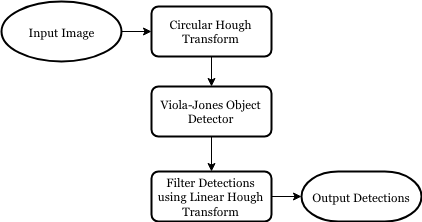
\includegraphics[width=0.8\linewidth]{images/flowdiagram.png}
\caption{Flow diagram of image detection algorithm. }
\label{default}
\end{center}
\end{figure}

\begin{figure}[htb]
\centering
\begin{subfigure}{.5\linewidth}
  \centering
  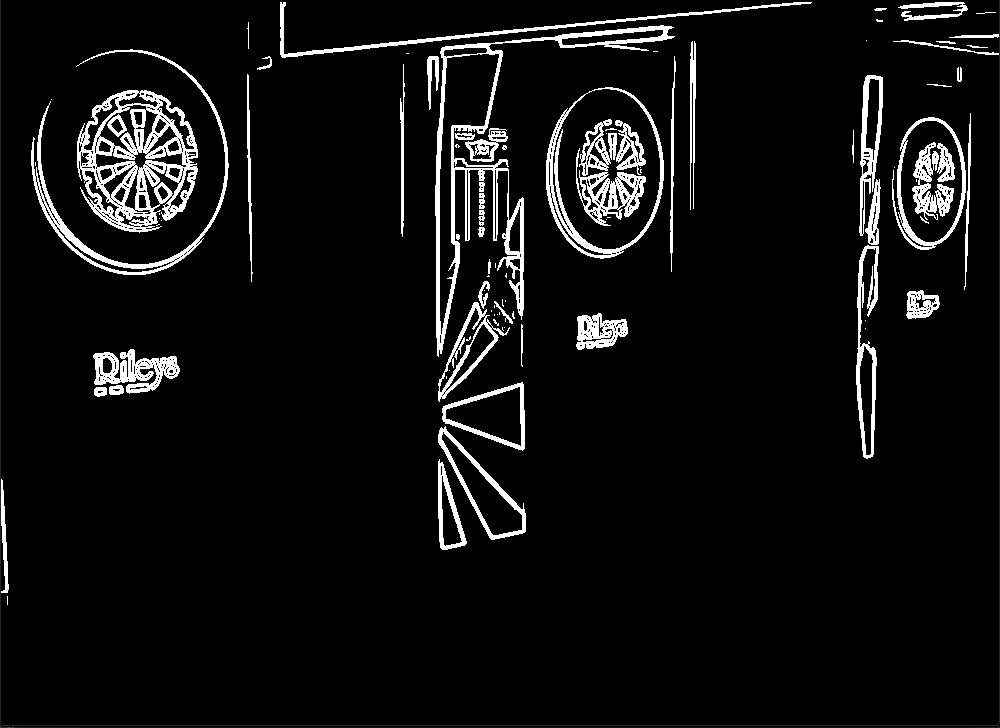
\includegraphics[width=.9\linewidth]{images/task3/bestthresh.png}
  \caption*{Gradient threshold}
  \label{fig:sub1}
\end{subfigure}%
\begin{subfigure}{.5\linewidth}
  \centering
  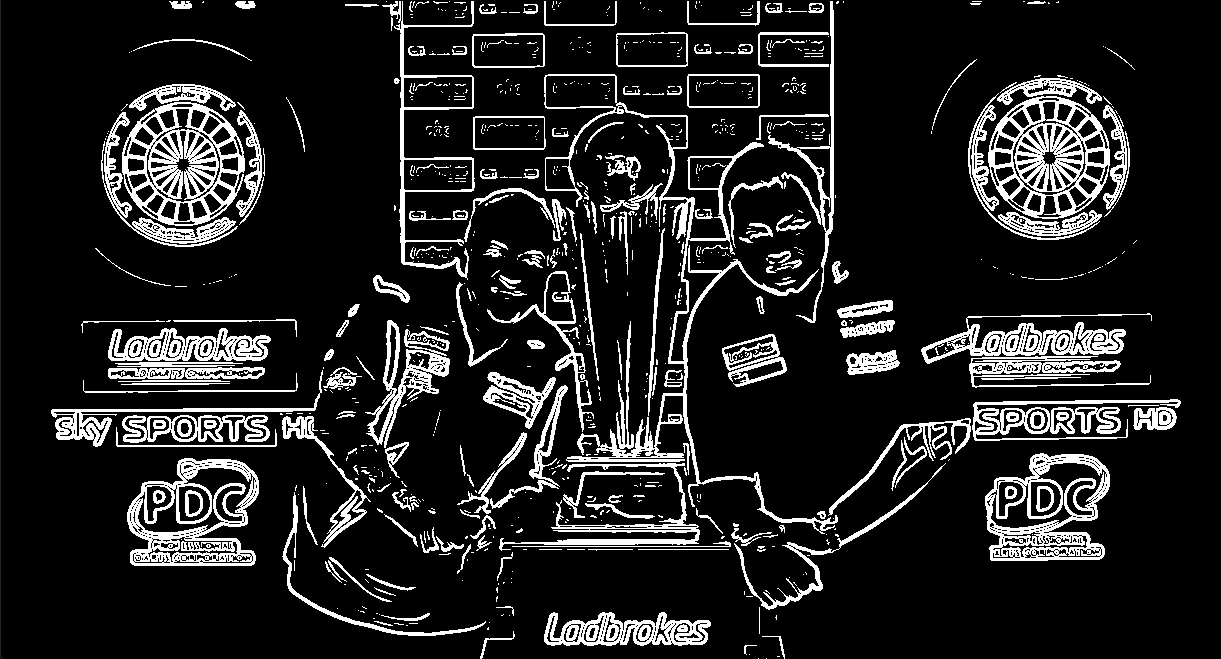
\includegraphics[width=.9\linewidth]{images/task3/worstthresh.png}
  \caption*{Gradient threshold}
  \label{fig:sub2}
\end{subfigure}
\begin{subfigure}{.5\linewidth}
  \centering
  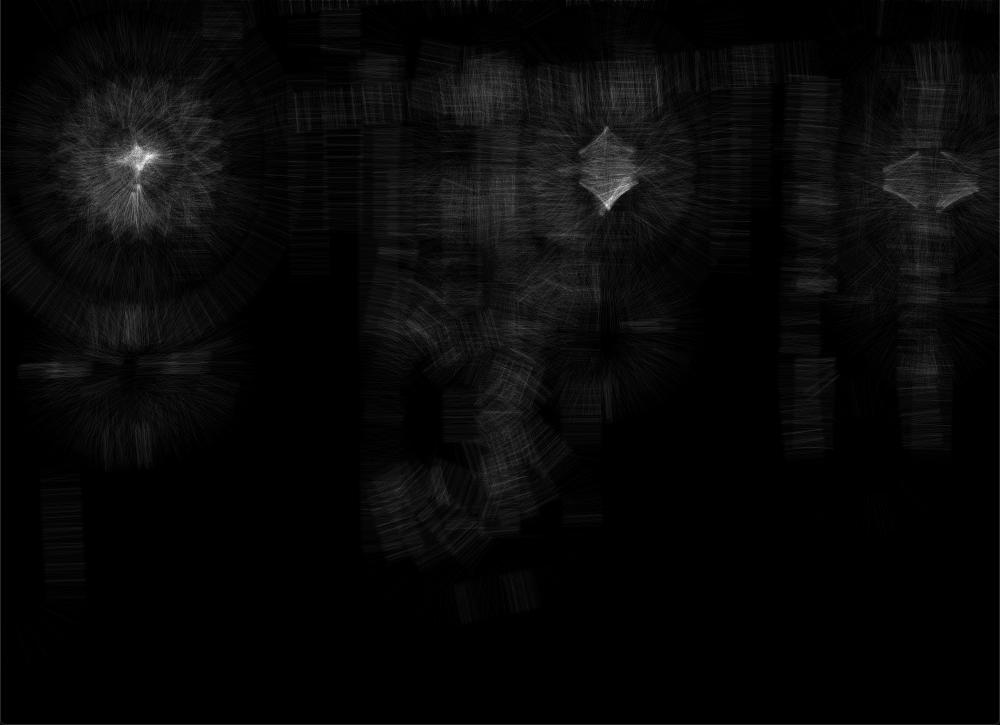
\includegraphics[width=.9\linewidth]{images/task3/bestcirclehough.png}
  \caption*{Circular Hough Transform}
  \label{fig:sub1}
\end{subfigure}%
\begin{subfigure}{.5\linewidth}
  \centering
  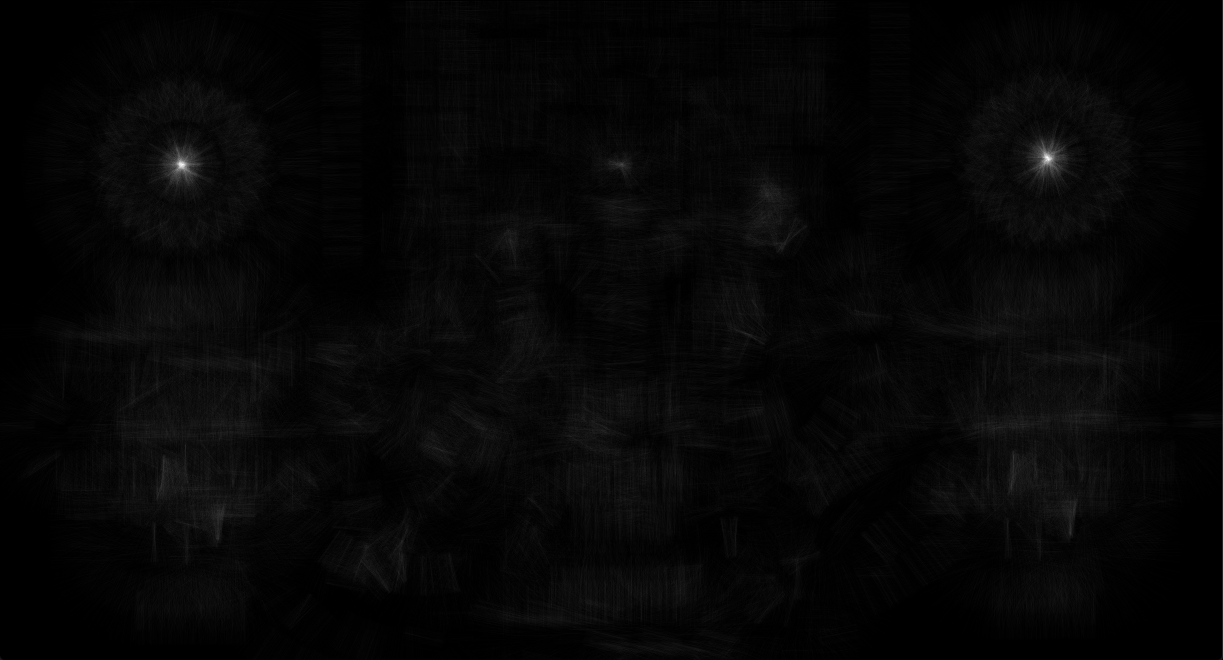
\includegraphics[width=.9\linewidth]{images/task3/worstcirclehough.png}
  \caption*{Circular Hough Transform}
  \label{fig:sub2}
\end{subfigure}
\begin{subfigure}{.5\linewidth}
  \centering
  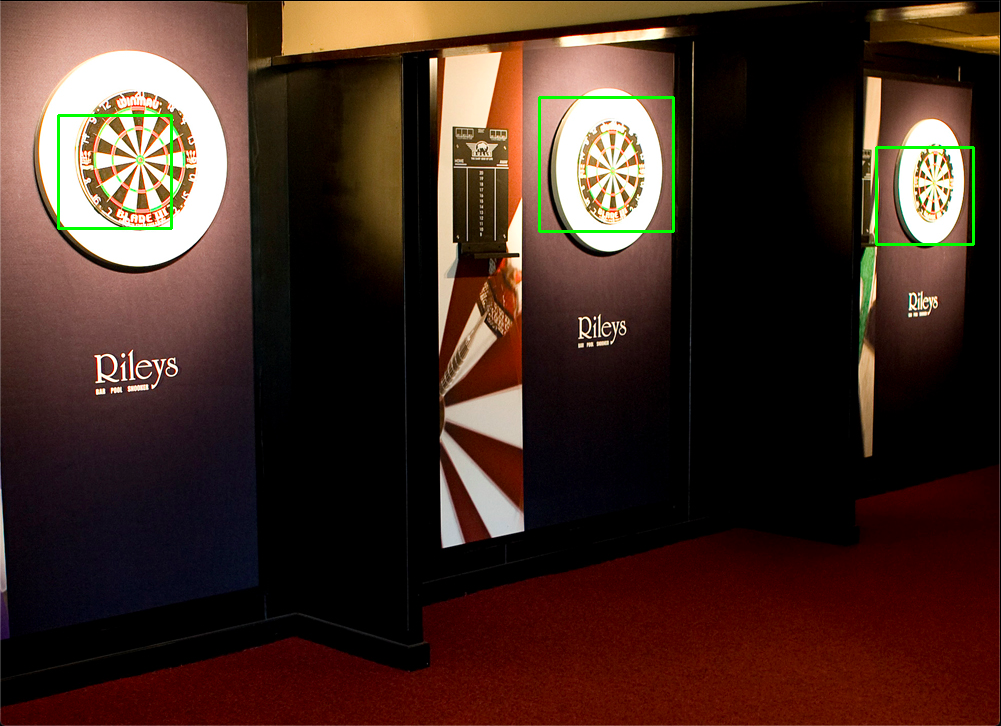
\includegraphics[width=.9\linewidth]{images/task3/bestresult.png}
  \caption{Detected Area}
  \label{fig:sub1}
\end{subfigure}%
\begin{subfigure}{.5\linewidth}
  \centering
  
\includegraphics[width=.9\linewidth]{images/task3/worstresult.png}
  \caption{Detected Area}
  \label{fig:sub2}
\end{subfigure}
\caption{Best and worst cases for the dartboard detector. Column a shows the best case, and has a F1 score of 1.  Column b shows the worst case is the worst case, and has an F1 score of 0.667}
\end{figure}
The rationale for building the classifier in this way include: 
\begin{itemize}
\item A circular hough transform is used to find circular features in the image;
\item The Viola-Jones object detector then determines if there are dartboards in the important area of the image;
\item Using the linear version of the hough transform allow for false detections to be filtered out.
\end{itemize}
\newpage
\par
The solution at this level gives very good results, achieving a true positive rate of 1 for all images. Only images 9 and 14 have imperfect F1 scores, caused by false positives. Image 9 could be considered to be a true positive as the classifier has detected a dartboard on a t-shirt. 




\newpage
\section{Further Improvements}






\end{document}